\documentclass[beamer]{standalone}
\usepackage{circuitikz}
\begin{document}

\title[Electronics 1]{Review Chapters 1--4}

\begin{frame} 
  \titlepage
\end{frame}

\section{Voltage divider}
\begin{frame}
 \frametitle{Unloaded voltage divider}
 \begin{columns}[c]
  \begin{column}{.3\textwidth}
   \begin{figure}
    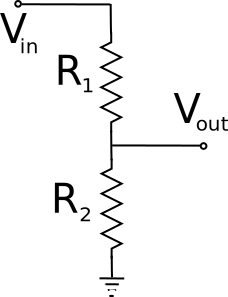
\includegraphics[height=2in]{./pics/unloaded_voltage_divider}
   \end{figure}
  \end{column}
  \begin{column}{.7\textwidth}
   \[ V_{out} = V_{in} \frac{R_2}{R_1+R_2} \]
  \end{column}
 \end{columns}
\end{frame}

\begin{frame}
 \frametitle{Loaded voltage divider}
 \begin{columns}[c]
  \begin{column}{.3\textwidth}
   \begin{figure}
    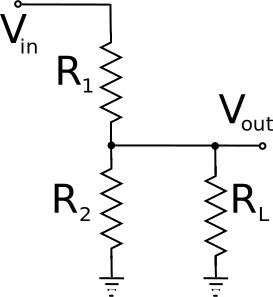
\includegraphics[height=2in]{./pics/loaded_voltage_divider}
   \end{figure}
  \end{column}
  \begin{column}{.7\textwidth}
   \[ V_{out,loaded} = V_{in} \frac{R_2}{R_1+R_2} \frac{R_L}{R_L + R_{1||2}} \]
   \[ V_{out,loaded} = V_{out,unloaded} \frac{R_L}{R_L + R_{1||2}} \]
  \end{column}
 \end{columns}
\end{frame}

\section{Th\'evenin's and Norton's  theorems}
\begin{frame}
 \frametitle{Th\'evenin's and Norton's equivalent circuit theorems}
	Any combination of voltage sources, current sources and resistors with
	two terminals is electrically equivalent 	
	\begin{columns}[t]
		\begin{column}{.45\textwidth}
			\begin{block} {Th\'evenin's theorem}
				to a single voltage source
				$V_{th}$ and a single series resistor $R_{th}$ connected in series.
			\end{block}
			\begin{figure}
				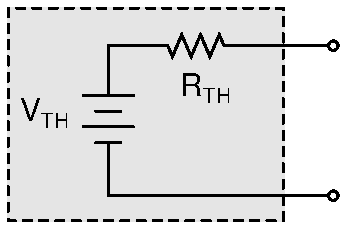
\includegraphics[width=0.55\textwidth]{./circuits/thevenin_circuit}
			\end{figure}
		\end{column}
		\begin{column}{.45\textwidth}
			\begin{block} {Norton's theorem}
				to a single current source
				$I_{N}$ and a single series resistor $R_{N}$ connected in parallel.
			\end{block}
			\begin{figure}
				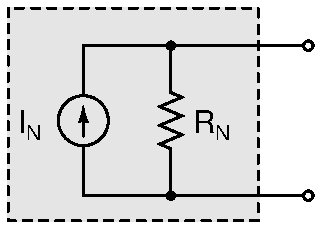
\includegraphics[width=0.55\textwidth]{./circuits/norton_circuit}
			\end{figure}
		\end{column}
	\end{columns}

	\center Note above circuits are equivalent to each other when\\
	\center $R_{th} = R_N$ and $I_N = V_{th}/R_{th}$
\end{frame}

\section{$I-V$ Diagrams}
\begin{frame}
 \frametitle{$I-V$ Diagrams}
 \begin{columns}[T]
  \begin{column}{0.6\textwidth}
   \begin{block}{Construct $I-V$ diagram}
    \begin{itemize}
     \item Change $R_{var}$ to change current
     \item Measure voltage across $R_{var}$
    \end{itemize}
   \end{block}
   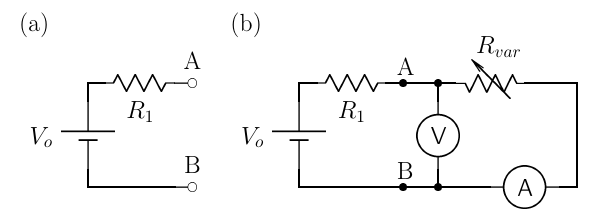
\includegraphics[width=\textwidth]{./pics/IV_circuit}
  \end{column}
  \begin{column}{0.4\textwidth}
   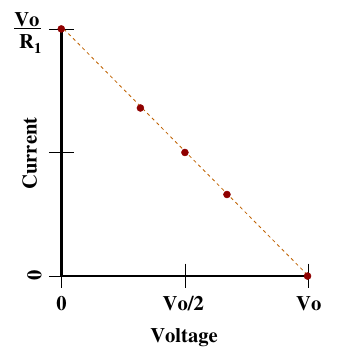
\includegraphics[width=\textwidth]{./pics/IV_Thevenin}
  \end{column}
 \end{columns}
 Notice when larger current drawn, smaller voltage maintained.
\end{frame}

\section{Voltage divider}
\begin{frame}
\frametitle{Voltage Divider}
\begin{columns}[t]
 \begin{column}{.45\textwidth}
  \begin{block}{Unloaded}
   \begin{figure}
    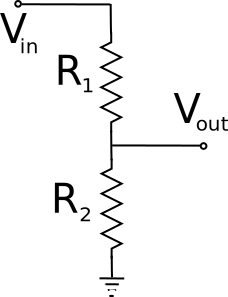
\includegraphics[height=1.5in]{./pics/unloaded_voltage_divider}
   \end{figure}
   \[ V_{out} = V_{in} \frac{R_2}{R_1+R_2} \]
  \end{block}
 \end{column}
  \begin{column}{.45\textwidth}
  \begin{block}{Loaded}
   \begin{figure}
    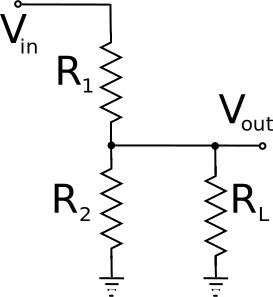
\includegraphics[height=1.5in]{./pics/loaded_voltage_divider}
   \end{figure}
   \[ V_{out} = V_{in} \frac{R_2}{R_1+R_2} \frac{R_L}{R_L + R_{1||2}} \]
   \[ V_{out} = V_{out,unloaded} \frac{R_L}{R_{1||2} + R_L} \]
  \end{block}
 \end{column}
\end{columns}
\end{frame}

\begin{frame}
 \frametitle{Voltage Divider: Power Dissipation}
 \begin{block}{Th\'evenin equivalent of unloaded voltage divider}
  Determine the Th\'evenin equivalent circuit:
  \begin{itemize}
   \item Open-circuit voltage is $V_{th} = V_{in} \frac{R_2}{R_1+R_2}$
   \item Short-circuit current is $I_{N} = \frac{V_{in}}{R_1} = \frac{V_{th}}{R_{th}}$
  \end{itemize}
  Th\'evenin resistance $R_{th} = \frac{V_{th}}{I_{N}} = R_{1||2}$
 \end{block}
 \begin{block}{Equivalent circuit of loaded voltage divider}
  Becomes very simple diagram with $V_{th}$ in series with $R_{th}$ and $R_{L}$
 \end{block}
\end{frame}

\section{Complex Impedances}
\begin{frame}
 \frametitle{Complex Impedances}
 \begin{block}{Impedance $Z$ of common components}
  \begin{center}
   \begin{tabular}{c|c|l|l}
    resistor & R & \\
    capacitor & $\frac{1}{j\omega C}$ & open for $\omega \to 0$ & short for $\omega \to \infty$ \\
    inductor & $j\omega L$ & short for $\omega \to 0$ & open for $\omega \to \infty$ \\
   \end{tabular}
  \end{center}
 \end{block}
\end{frame}

\begin{frame}
 \frametitle{Gain of a Circuit}
 \begin{block}{Limits of gain in an RC-circuit}
  \begin{columns}
   \begin{column}{0.0\textwidth}
   \end{column}
   \begin{column}{0.5\textwidth}
    \pgfimage[width=\textwidth]{pics/RC_filter}
   \end{column}
   \begin{column}{0.5\textwidth}
    \begin{equation*}
     G(\omega) = \frac{1}{1 + j\omega R C}
    \end{equation*}
   \end{column}
  \end{columns}
  \begin{itemize}
   \item Low frequency $\omega \ll \frac{1}{RC}$: $G(\omega) \approx 1$ (DC limit)
   \item High frequency $\omega \gg \frac{1}{RC}$: $G(\omega) \approx \frac{1}{j\omega R C} \approx 0$
  \end{itemize}
 \end{block}
 \begin{block}{Bode plots}
  \begin{center}
   \pgfimage[width=0.4\textwidth]{pics/Bode_plot}
  \end{center}
 \end{block}
\end{frame}

\begin{frame}
\frametitle{Bode plots}
 \begin{block}{What are Bode plots?}
  Plots of magnitude and phase of the transfer function, where
  $|G|$ is often plotted in dB
 \end{block}
   \begin{columns}[c]
    \begin{column}{.25\textwidth}
     \begin{figure}
      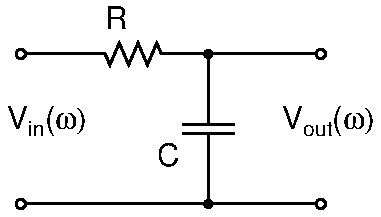
\includegraphics[width=1.00\textwidth]{./circuits/rc_low_pass.pdf}
     \end{figure}
    \[ G(\omega)
    = \frac{1}{1+j\frac{\omega}{\omega_{3dB}}}
    \]
    \end{column}
    \begin{column}{.75\textwidth}
      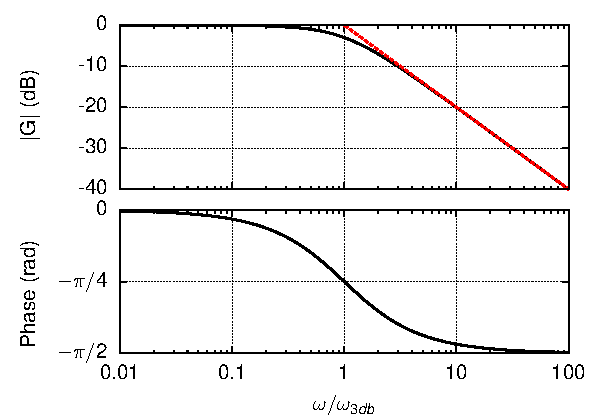
\includegraphics[angle=0,width=1.00\textwidth]{./plots/rc_low_pass_bode.pdf}
    \end{column}
   \end{columns}
\end{frame}

\begin{frame}
 \frametitle{Filters chain}
 \begin{figure}
  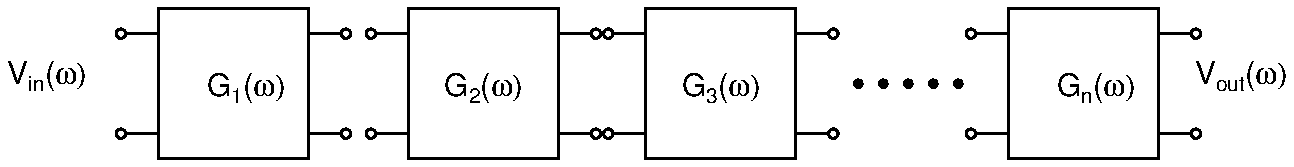
\includegraphics[angle=0,width=1.0\textwidth]{./circuits/black_box_transfer_in_freq_chain.pdf}
 \end{figure}
 Technically next stage loads the previous and it is quite hard to
 calculate total transfer function.

 However we use rule of 10 to avoid overloading the previous filter.\\
 Every next stage resistor $|Z_{in,i+1}| > 10 |Z_{out,i}|$ we can approximate
 \[
 G_t(\omega) \approx G_1(\omega) G_2(\omega) G_3(\omega) \cdots G_n(\omega)
 \]
\end{frame}


\section{Diodes}
\begin{frame}
\frametitle{Real diode}
\vskip -.2in
\begin{figure}
  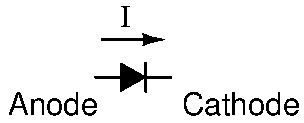
\includegraphics[width=0.30\textwidth]{./schematics/diode}
\end{figure}

\vskip -.2in
\begin{columns}[t]
  \begin{column}{.35\textwidth}
    \[
    I(V)=I_S\left( e^{{V}/(m V_{T})}-1 \right) 
    \]
    Typical parameters
    \begin{itemize}
      \item saturation current $I_S=1$~nA
      \item thermal voltage $V_T=\frac{kT}{q}=25.85$~mV at 300~K
      \item emission coefficient $m=1..2$
    \end{itemize}
    
  \end{column}
  \begin{column}{.65\textwidth}
    \begin{figure}
      \includegraphics<1>[angle=0,width=1.00\textwidth]{./plots/realistic_diode}
      \includegraphics<2>[angle=0,width=1.00\textwidth]{./plots/diode_combined}
    \end{figure}
  \end{column}
\end{columns}
\end{frame}

\section{Full-wave rectifier}
\begin{frame}
 \frametitle{Full-wave rectifier: $V_{in} \gg V_d \to V_{out} \approx | V_{in}|$}
  \begin{columns}[c]
    \begin{column}{.50\textwidth}
  \begin{figure}
    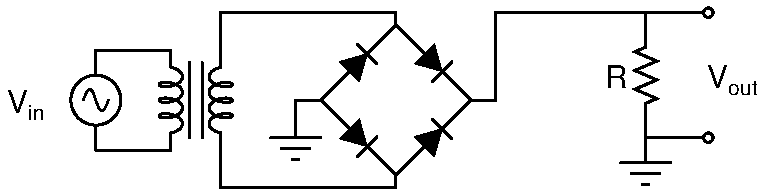
\includegraphics[width=0.90\columnwidth]{./schematics/full_wave_rectifier}
  \end{figure}
    \end{column}
    \begin{column}{.50\textwidth}
      Why $\max(V_{out}) = V_0 - \alert{2 V_d} $ ? \\
      Why transformer?
    \end{column}
  \end{columns}
  %\vskip -.5in
    \begin{figure}
      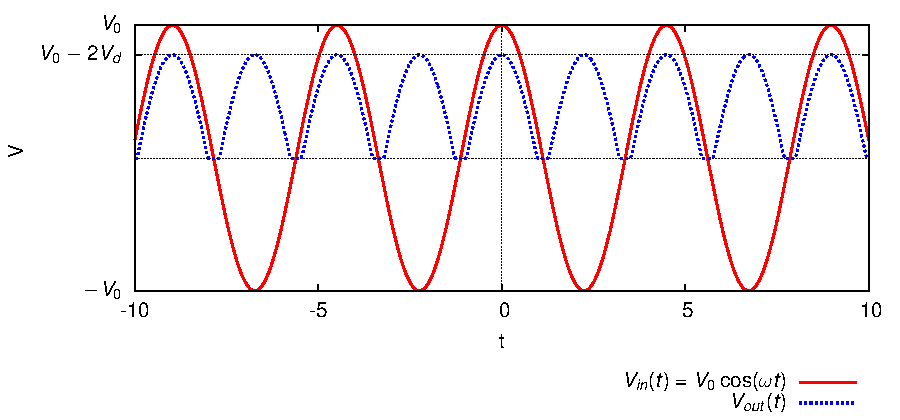
\includegraphics[angle=0,width=1.00\columnwidth]{./plots/full_wave_rectifier}
    \end{figure}
\end{frame}



\section{RLC filters}
\begin{frame}
 \frametitle{RLC filters}
 \begin{columns}
  \begin{column}{0.4\textwidth}
   \pgfimage[width=\textwidth]{pics/RLC_circuit}
  \end{column}
  \begin{column}{0.6\textwidth}
   \begin{itemize}
    \item $\omega_{LC} = \frac{1}{\sqrt{LC}}$
    \item $\omega_{RC} = \frac{1}{RC}$
    \item $\omega_{RL} = \frac{R}{L}$
   \end{itemize}
   Note: $\omega_{RC} \omega_{RL} = \omega^2_{LC}$
  \end{column}
 \end{columns}
 \begin{block}{Three output voltages}
  \begin{columns}
   \begin{column}{0.5\textwidth}
    \begin{itemize}
     \item $v_o^R(\omega)$ across resistor
     \item $v_o^L(\omega)$ across inductor
     \item $v_o^C(\omega)$ across capacitor
    \end{itemize}
   \end{column}
   \begin{column}{0.5\textwidth}
    Typically $R$ and $L$ in one component, so measure $v_o^R(\omega) + v_o^L(\omega)$
   \end{column}
  \end{columns}
 \end{block}
\end{frame}

\begin{frame}
 \frametitle{RLC filters}
 \begin{block}{Total impedance}
  \begin{equation*}
   Z_{tot} = R + j\omega L + \frac{1}{j\omega C} = R \left[ 1 - j\frac{\omega_{RC}}{\omega} \left( 1 - \frac{\omega^2}{\omega_{LC}^2} \right) \right]
  \end{equation*}
 \end{block}
 \begin{block}{Voltage divider: gain across capacitor}
  \begin{equation*}
   G_C(\omega) = \frac{Z_C}{Z_{tot}} = \frac{1}{j\omega RC\left[ 1 - j\frac{\omega_{RC}}{\omega} \left( 1 - \frac{\omega^2}{\omega_{LC}^2} \right) \right]} = \frac{1}{\left( 1 - \frac{\omega^2}{\omega_{LC}^2} \right) + j\frac{\omega}{\omega_{RC}}}
  \end{equation*}
  \begin{eqnarray*}
   |G_C(\omega)| & = & \frac{1}{\sqrt{ \left(1 - \omega^2/\omega_{LC}^2 \right)^2 + \omega^2/\omega^2_{RC}}} \\
   \phi_C & = & \tan^{-1} \frac{- \omega/\omega_{RC}}{1 - \omega^2/\omega_{LC}^2}
  \end{eqnarray*}
 \end{block}
\end{frame}

\begin{frame}
 \frametitle{RLC filters: gain across capacitor}
 \begin{block}{Resonance at $\omega = \omega_{LC}$}
  \begin{itemize}
   \item $|G_C(\omega)| = \frac{\omega_{RC}}{\omega_{RL}} = \sqrt{\frac{L}{R^2 C}}$ large for $R$ small
   \item $\phi_C = -\frac{\pi}{2}$
  \end{itemize}
 \end{block}
 \begin{block}{Low frequency limit}
  \begin{itemize}
   \item $|G_C(\omega)| \to 1$
   \item $\phi_C \to 0$
  \end{itemize}
 \end{block}
 \begin{block}{High frequency limit}
  \begin{itemize}
   \item $|G_C(\omega)| \to \frac{\omega^2_{LC}}{\omega^2}$
   \item $\phi_C \to -\pi$
  \end{itemize}
 \end{block}
\end{frame}

\begin{frame}
 \frametitle{RLC filters: gain across capacitor}
 \begin{center}
  \pgfimage[width=0.6\textwidth]{pics/RLC_bode_capacitor}
 \end{center}
\end{frame}

\begin{frame}
 \frametitle{RLC filters}
 \begin{block}{Voltage divider: gain across inductor}
  \begin{equation*}
   G_L(\omega) = \frac{Z_L}{Z_{tot}} = \frac{j\omega L}{R\left[ 1 - j\frac{\omega_{RC}}{\omega} \left( 1 - \frac{\omega^2}{\omega_{LC}^2} \right) \right]} = \frac{1}{\left( 1 - \frac{\omega^2_{LC}}{\omega^2} \right) + j\frac{\omega_{RL}}{\omega}}
  \end{equation*}
  \begin{eqnarray*}
   |G_L(\omega)| & = & \frac{1}{\sqrt{ \left(1 - \omega_{LC}^2/\omega^2 \right)^2 + \omega_{RL}^2/\omega^2}} \\
   \phi_L & = & \tan^{-1} \frac{\omega_{RL}/\omega}{1 - \omega_{LC}^2/\omega^2}
  \end{eqnarray*}
 \end{block}
\end{frame}

\begin{frame}
 \frametitle{RLC filters: gain across inductor}
 \begin{block}{Resonance at $\omega = \omega_{LC}$}
  \begin{itemize}
   \item $|G_L(\omega)| = \frac{\omega_{LC}}{\omega_{RL}} = \sqrt{\frac{L}{R^2 C}}$ large for $R$ small
   \item $\phi_L = \frac{\pi}{2}$
  \end{itemize}
 \end{block}
 \begin{block}{Low frequency limit}
  \begin{itemize}
   \item $|G_L(\omega)| \to \frac{\omega^2}{\omega_{LC}^2}$
   \item $\phi_L \to \pi$
  \end{itemize}
 \end{block}
 \begin{block}{High frequency limit}
  \begin{itemize}
   \item $|G_L(\omega)| \to 1$
   \item $\phi_L \to 0$
  \end{itemize}
 \end{block}
\end{frame}

\begin{frame}
 \frametitle{RLC filters: gain across inductor}
 \begin{center}
  \pgfimage[width=0.6\textwidth]{pics/RLC_bode_inductor}
 \end{center}
\end{frame}

\begin{frame}
 \frametitle{RLC filters: gain larger than 0\,dB}
 \begin{columns}
  \begin{column}{0.5\textwidth}
   \pgfimage[width=\textwidth]{pics/RLC_bode_capacitor}   
  \end{column}
  \begin{column}{0.5\textwidth}
   \pgfimage[width=\textwidth]{pics/RLC_bode_inductor}
  \end{column}
 \end{columns}
 \begin{block}{Gain larger than 1}
  Possible when the phase is opposite:
  \begin{itemize}
   \item $v_C(t) + v_L(t) = 0$
  \end{itemize}
 \end{block}
\end{frame}

\end{document}
